\documentclass[a4paper]{article}
\usepackage[utf8]{inputenc}
\usepackage[russian,english]{babel}
\usepackage[T2A]{fontenc}
\usepackage[left=10mm, top=20mm, right=18mm, bottom=15mm, footskip=10mm]{geometry}
\usepackage{indentfirst}
\usepackage{amsmath,amssymb}
\usepackage[italicdiff]{physics}
\usepackage{graphicx}
\graphicspath{{images/}}
\DeclareGraphicsExtensions{.pdf,.png,.jpg}
\usepackage{wrapfig}
\usepackage{pgfplots}

\usepackage{caption}
\captionsetup[figure]{name=Рисунок}
\captionsetup[table]{name=Таблица}


\title{\underline{Лабораторная работа 2.1.1}}
\author{Старостин Александр, Б01-401}
\date {12 Марта, 2025 год}


\begin{document}

\maketitle
\newpage

\textbf{Измерение удельной теплоёкости теплоёмкости воздуха при постоянном давлении}

\section{Аннотация}
    \par \textbf{Цель работы:} измерить повышение температуры воздуха в зависимости от мощности подводимого тепла и расхода при стационарном течении через трубу; исключив тепловые потери, по результатам измерений определить теплоёмкость воздуха при постоянном давлении. \\

    \par \textbf{В работе используются:} теплоизолированная стеклянная трубка; электронагреватель; источник питания постоянного тока; амперметр, вольтметр (цифровые мультиметры); термопара, подключенная к микровольтметру; компрессор; газовый счётчик;
	секундомер.

\section{Теоретические сведения}

    Теплоёмкость тела в некотором процессе определяется как их отношение: 
	\begin{equation*}
		C = \frac{\delta Q}{dT}
		\eqno(1)
	\end{equation*}
	
	Необходимо, чтобы количество тепла, затрачиваемое на нагревание исследуемого тела, существенно превосходило тепло, расходуемое на нагревание самого калориметра, а также на потери тепла из установки.
	
	Для увеличения количества нагреваемого газа при неизменных размерах установки в нашей работе исследуемый газ (воздух) продувается через калориметр, внутри которого установлен нагреватель. При этом
	измеряются мощность нагревателя, масса воздуха, протекающего в единицу
	времени (расход), и приращение его температуры.
	
	\begin{figure}[h!]
		\centering{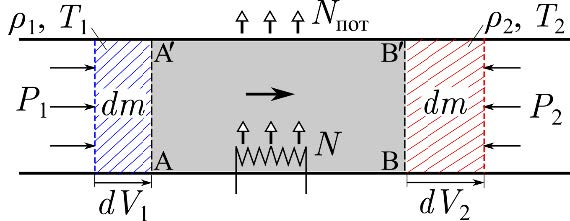
\includegraphics[width=0.5\textwidth]{pic2.jpg}}
		\caption[]{\label{fig:1} Нагрев газа при течении по трубе}
	\end{figure}

	Рассмотрим газ, протекающий стационарно слева направо через трубу постоянного сечения, в которой установлен нагревательный элемент (см. рис. 1). Пусть за некоторое время $dt$ через калориметр прошла малая порция газа массой $dm=q \, dt$, где $q$ [кг/с] — массовый расход газа в трубе. Если мощность нагрева равна $N$, мощность тепловых потерь на обмен с окружающей средой $N_{пот}$, то порция
	получила тепло $\delta Q = (N-N_{пот})dt$. С другой стороны, по определению теплоёмкости (1): $\delta Q = c \, dm \Delta T$, где $\Delta T = T_{2}-T_{1}$ — приращение температуры	газа, и $c$ — удельная (на единицу массы) теплоёмкость газа в рассматриваемом процессе. При малых расходах газа и достаточно большом диаметре
	трубы перепад давления на её концах мал, поэтому можно принять, что $P_{1} \approx P_{2} = P_{0}$, где $P_{0}$ — атмосферное давление. Следовательно, в условиях опыта
	измеряется удельная теплоёмкость при постоянном давлении $c_{P}$. Таким образом, получаем 
	\begin{equation*}
		c_{P} = \frac{N-N_{пот}}{q\Delta T}
		\eqno(2)
	\end{equation*}
	
	\subparagraph*{Экспериментальная установка:}
	
	Схема установки изображена на рис. 2. Воздух, нагнетаемый компрессором, прокачивается через калориметр. Калориметр представляет собой стеклянную цилиндрическую трубку с двойными стенками, запаянными с торцов.
	
	\begin{figure}[h!]
		\centering{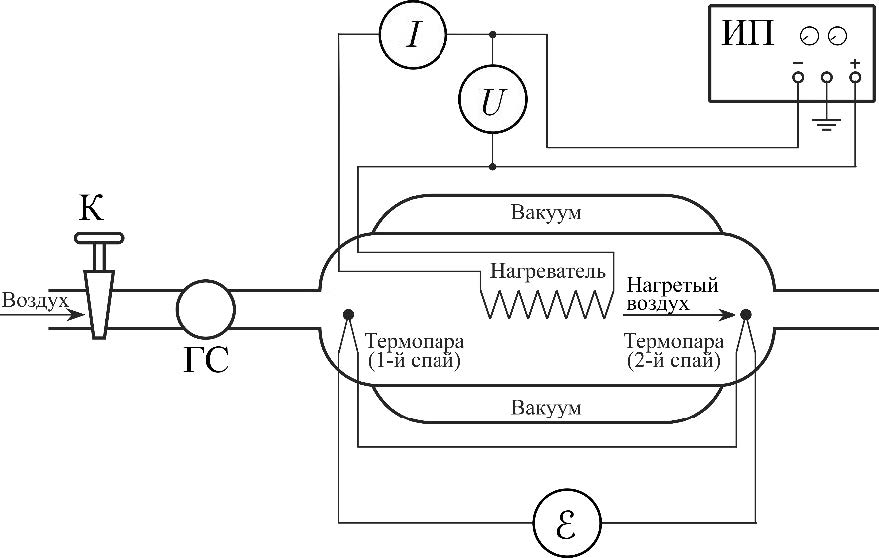
\includegraphics[width=0.5\textwidth]{pic3.jpg}}
		\caption[]{\label{fig:2} Схема экспериментальной установки}
	\end{figure}

	
	Нагреватель в виде намотанной на пенопласт нихромовой проволоки расположен внутри калориметра непосредственно в воздушном потоке. Нагрев проволоки производится от регулируемого источника постоянного тока (ИП).
	Напряжение $U$ на нагревателе и ток $I$ через него регистрируются цифровыми мультиметрами. Таким образом, мощность нагрева равна
	\begin{equation*}
		N = UI
		\eqno(3)
	\end{equation*}

	Для измерения разности температур $\Delta T$ служит медно-константановая
	термопара. Один спай термопары расположен в струе воздуха, входящего в
	калориметр, и находится при комнатной температуре, а второй — в струе выходящего нагретого воздуха. Константановая проволока термопары расположена внутри калориметра, а медные проводники подключены к цифровому вольтметру. Возникающая в термопаре ЭДС $\varepsilon$ пропорциональна разности температур $\Delta T$ спаев: 
	\begin{equation*}
		\varepsilon =\beta \Delta T
		\eqno(4)
	\end{equation*}

	где $\beta = 40.7 \frac{мкВ}{К}$ — чувствительность медно-константановой термопары в рабочем диапазоне температур (20–30 $^\circ C$ ). ЭДС регистрируется с помощью микровольтметра.
	
	Объём воздуха, прошедшего через калориметр, измеряется газовым счётчиком ГС. Для регулировки расхода служит кран К. Время $\Delta t$ прохождения
	некоторого объема $\Delta V$ воздуха измеряется секундомером. Объёмный расход равен $\frac{\Delta V}{\Delta t} $, массовый расход может быть найден как 
	\begin{equation*}
		q = \rho_{0} \frac{\Delta V}{\Delta t}
		\eqno(5)
	\end{equation*}
	
	где $\rho_{0}$ — плотность воздуха при комнатной температуре, которая в свою очередь может быть получена из уравнения Менделеева–Клапейрона: $\rho_{0}= \frac{\mu P_{0} }{R T_{0}},$ где $P_{0}$ — атмосферное давление, $T_{0}$ — комнатная температура (в Кельвинах), $\mu = 29,0 {г/моль}$ — средняя молярная масса (сухого) воздуха.
	
	Учитывая особенности устройства калориметра, следует ожидать, что мощность нагревателя расходуется не только на нагрев массы прокачиваемого воздуха, но и частично теряется за счет нагрева внутренних стенок термостата и рассеяния тепла через торцы термостата. Можно предположить, что при небольшом нагреве ($\Delta T \ll T_{0}$) мощность потерь тепла $N_{пот}$ прямо пропорциональна разности температур:
	\begin{equation*}
		N_{пот} = \alpha \Delta T
		\eqno(6)
	\end{equation*}
	
	где $\alpha$ — некоторая константа. При этом условии основное соотношение (2) принимает вид 
	\begin{equation*}
		N = (C_{P}q +\alpha)\Delta T
		\eqno(7)
	\end{equation*}

	Следовательно, при фиксированном расходе воздуха ($q = \const$) подводимая мощность и разность температур связаны прямой пропорциональностью ($\Delta T(N)$ -- линейная функция).


\section{Ход работы}


\end{document}














	
	